%%%%%%%%%%%%%%%%%%%%%%%%%%%%%%%%%%%%%%%%%%%%%%%%%%%%%%%%%%%%%%%%%%%%%%%%%%%%%%%%%%%%%%5
\section{Exploración Bivariada}\label{bivariada}


\begin{Schunk}
\begin{Soutput}
       cabeLog  restoLog
[1,] 0.4873974 0.1773112
\end{Soutput}
\begin{Soutput}
         cabeLog restoLog
cabeLog  "1"     ""      
restoLog "0.84"  "1"     
\end{Soutput}
\end{Schunk}
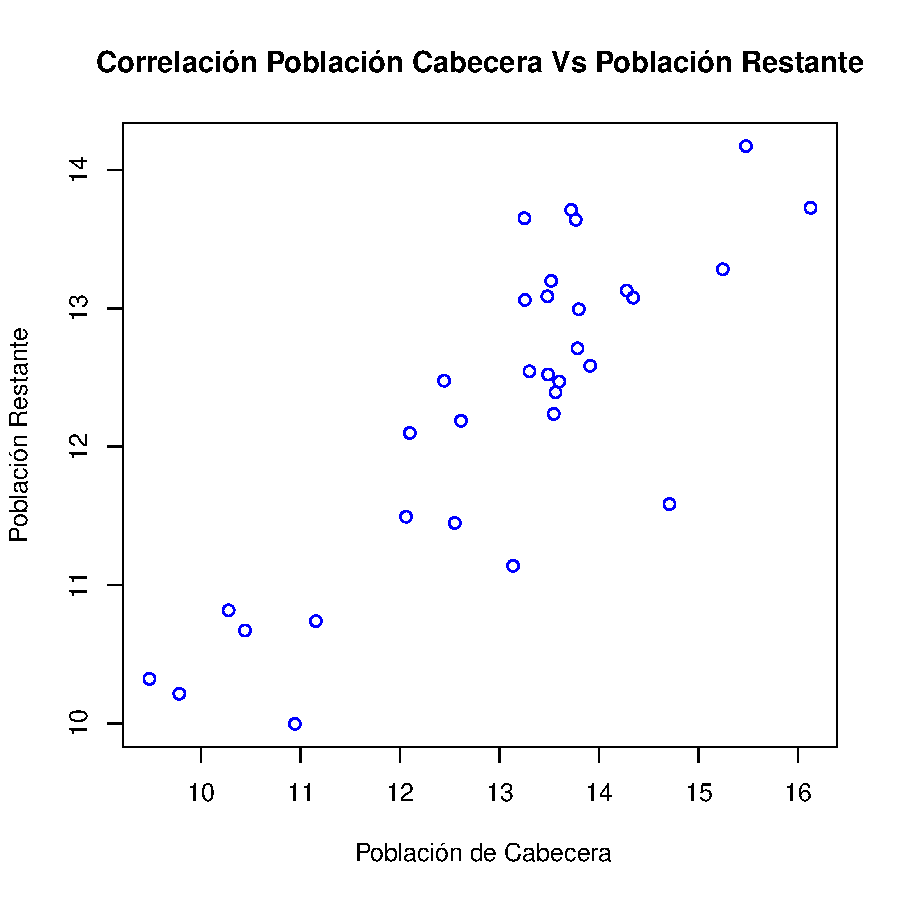
\includegraphics{bivariada-correl}

\endinput
